% !TeX spellcheck = en_US
% !TeX encoding = utf8
% !TeX program = xelatex
% !BIB program = bibtex

\documentclass[a4paper]{article}

\usepackage[english]{babel}
\usepackage[utf8]{inputenc}
\usepackage{amsmath}
\usepackage{graphicx}
\usepackage[colorinlistoftodos]{todonotes}

\title{Linear Optimization -- Homework 1}

\author{Due: Sunday, April, 1}

\date{}

\begin{document}
\maketitle

% \begin{abstract}
% 	Enter a short summary here. What topic do you want to investigate and why? What experiment did you perform? What were your main results and conclusion?
% \end{abstract}



\begin{figure}
	\centering
	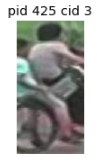
\includegraphics[width=0.3\textwidth]{frog.png}
	\caption{\label{fig:frog}This frog was uploaded to writeLaTeX via the project menu.}
\end{figure}


\end{document}